\begin{center}
    \vspace{2cm} 
    {\Huge \bfseries Abril} \\ 
    \vspace{1cm} 
\end{center}

\subsection*{Introdução}
Utilizamos o site \href{https://www.tinkercad.com}{Tinkercad} para nos familiarizarmos com a montagem do circuito. Nele, é possível criar um ambiente virtual no qual é possível testar ligações entre Arduino, resistores, lâmpadas, botões e outros componentes. Além disso, permite escrever e executar códigos em C\texttt{++}, proporcionando maior complexidade e possibilidades aos circuitos.\\

\subsubsection*{Prática realizada}
\noindent Criar um circuito com dois LEDs e dois botões.\\
\vspace{-0.2cm}
\begin{itemize}
    \item Apertar o botão 1 $\rightarrow$ LED 1 acende, LED 2 apaga
    \item Apertar o botão 2 $\rightarrow$ LED 2 acende, LED 1 apaga
\end{itemize}

\begin{figure}[h]
    \centering
    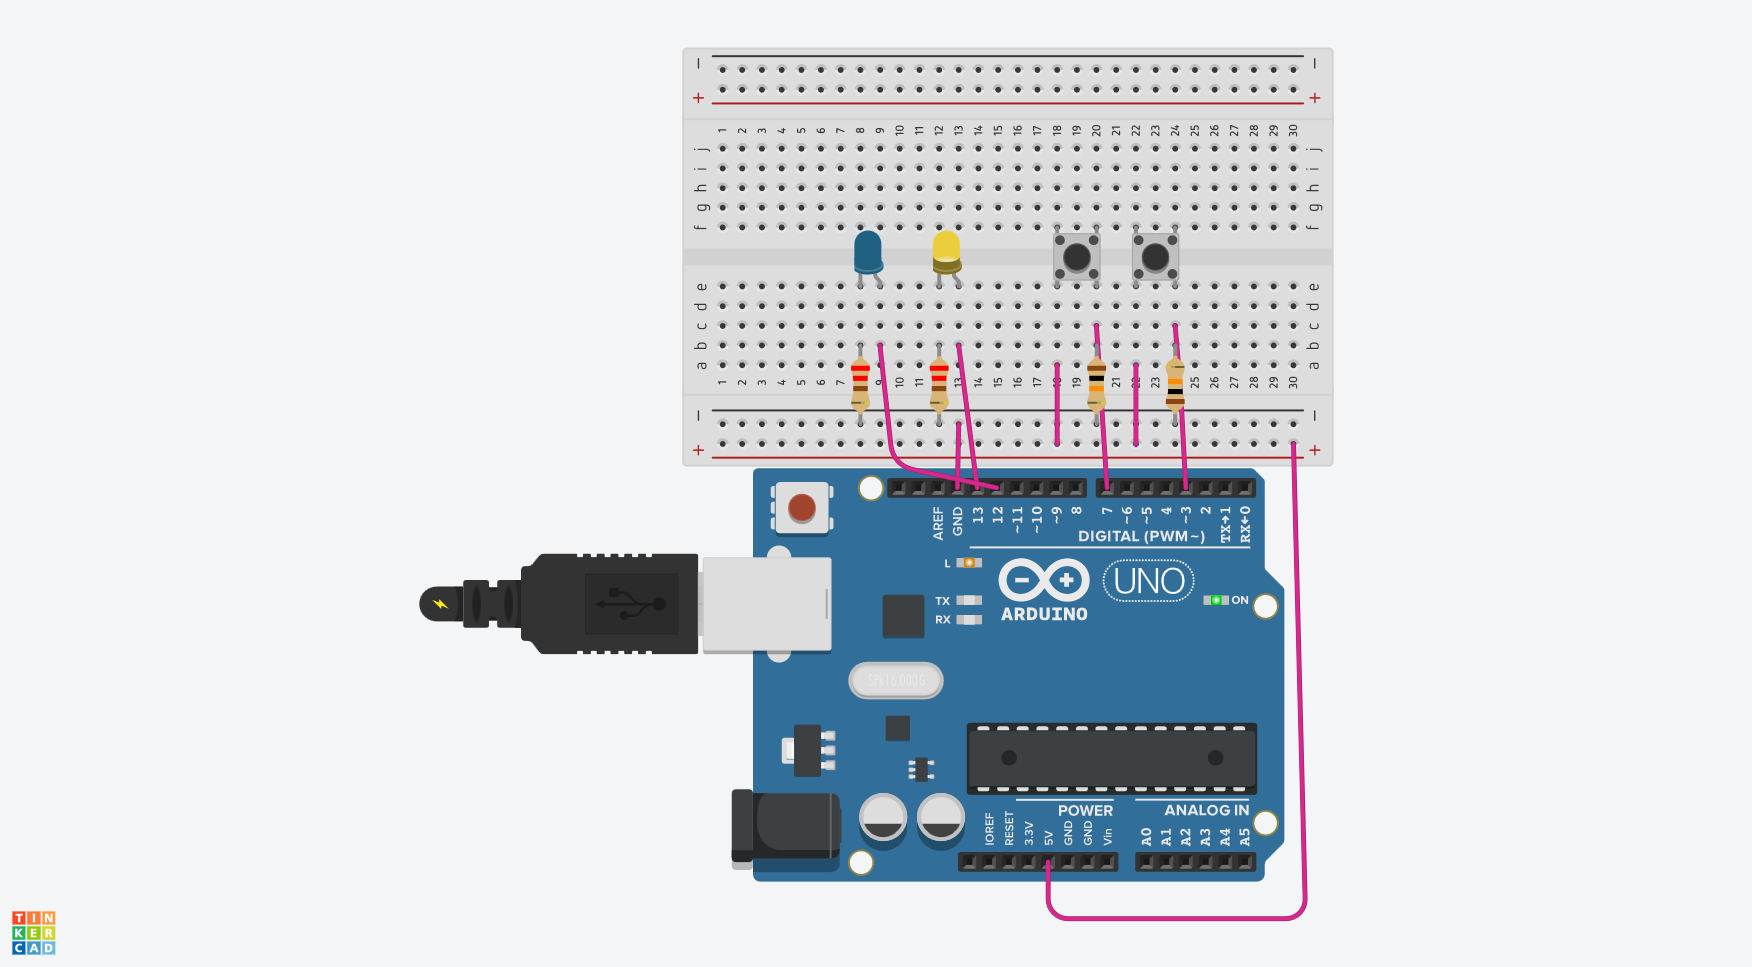
\includegraphics[width=1.0\textwidth]{./figs/pratica-arduino.png}
    \caption*{Circuito montado no Tinkercad.}
    \label{fig:circuito_arduino}
\end{figure}

\newpage

\lstinputlisting[title={C\'odigo-fonte do programa do Arduino}]{./codes/pratica_arduino.ino}
\bigbreak

\noindent Circuito no Tinkercad: \href{https://www.tinkercad.com/things/isqw31TJhYH-pratica-dois-botoes?sharecode=OD8YmILx-zFJkZS_fJNu8jKlsnR4dTg6y4rJ6c_sYVA}{Prática - dois botões} \\
\noindent Material de apoio utilizado: \href{https://www.blogdarobotica.com/2020/09/28/ligar-e-desligar-led-com-botao-push-button-chave-tactil-com-arduino/}{Blog da Robótica}.
